% ============================================================================
% Pedagogical solutions: Practice 5 - Combinatorics, basic rules.
% English, pdflatex. Source is ASCII-clean (no em-dashes, no curly quotes).
% Compile: pdflatex twice.
% ============================================================================
\documentclass[11pt,a4paper]{article}

% ---- Encoding & fonts ----
\usepackage[utf8]{inputenc}
\usepackage[T1]{fontenc}
\usepackage{lmodern}

% ---- Math ----
\usepackage{amsmath,amssymb,amsthm}
\usepackage{mathtools}

% ---- Layout ----
\usepackage[margin=2.3cm]{geometry}
\usepackage{enumitem}
\usepackage{booktabs}
\usepackage{array}

% ---- Visuals ----
\usepackage{xcolor}
\usepackage[most]{tcolorbox}
\usepackage{tikz}
\usetikzlibrary{arrows.meta,positioning,calc,fit,backgrounds,shapes.misc}
\usepackage{pgfplots}
\pgfplotsset{compat=1.18}
\usepackage{hyperref}
\hypersetup{colorlinks=true,linkcolor=blue!55!black,urlcolor=blue!55!black}

% ---- Palette (Armenian flag colours; use for 3+ series plots) ----
\definecolor{armRed}{HTML}{D90012}
\definecolor{armBlue}{HTML}{0033A0}
\definecolor{armOrange}{HTML}{F2A800}
\definecolor{ink}{HTML}{22303C}

\setlength{\parindent}{0pt}
\setlength{\parskip}{5pt}

% ---- Boxes ----
\newtcolorbox{problembox}[1][]{enhanced, breakable, sharp corners=south,
  colback=armOrange!10, colframe=armOrange!75!black, boxrule=0.8pt, arc=2mm,
  fonttitle=\bfseries\color{white}, coltitle=white,
  attach boxed title to top left={xshift=4mm,yshift=-2.4mm},
  boxed title style={colback=armOrange!85!black, arc=1mm},
  title={Problem #1}}

\newtcolorbox{ideabox}{enhanced, breakable,
  colback=armBlue!6, colframe=armBlue!70!black, boxrule=0.8pt, arc=2mm,
  fonttitle=\bfseries\color{white}, coltitle=white,
  attach boxed title to top left={xshift=4mm,yshift=-2.4mm},
  boxed title style={colback=armBlue!75!black, arc=1mm},
  title={The idea}}

\newtcolorbox{methodbox}{enhanced, breakable,
  colback=gray!8, colframe=gray!55!black, boxrule=0.7pt, arc=2mm,
  fonttitle=\bfseries, title={$\bigstar$\ Method to remember}}

\newtcolorbox{answerbox}{enhanced, sharp corners=south,
  colback=green!8, colframe=green!50!black, boxrule=1pt, arc=2mm, left=4mm,right=4mm}
\newcommand{\answer}[1]{\begin{answerbox}\centering\textbf{Answer:}\quad #1\end{answerbox}}

% ---- Title ----
\title{\vspace{-1.2cm}\textbf{Discrete Mathematics - Practical 5}\\[2pt]
\large Combinatorics, the basic counting rules: worked solutions\\[2pt]
\normalsize\itshape with the reasoning spelled out, step by step}
\author{}
\date{}

\begin{document}
\maketitle
\vspace{-1.0cm}

\section*{Warm-up}
This sheet is about \emph{counting without listing}. Almost everything here rests on two rules.
The \textbf{product rule}: if a thing is built by making a first choice in $a$ ways and then,
independently, a second choice in $b$ ways, there are $a\cdot b$ ways in total (a grid with $a$
rows and $b$ columns). The \textbf{sum rule}: if a thing falls into separate, non-overlapping
cases with $a$ and $b$ options, there are $a+b$ options in total. Two later problems add the
\textbf{pigeonhole principle}: if you put $n+1$ objects into $n$ boxes, some box holds at least
two. Counting is visual - draw the slots, the cases, or the boxes, and the formula reads itself
off the picture. We solve sections 1 and 2 problems labelled 1.3, 1.5, 1.10, 2.5, 2.10, 2.12.

% ============================================================================
\section*{Problem 1.3 - Two books of different subjects}

\begin{problembox}[1.3]
A shelf has $15$ informatics books, $12$ mathematics books, and $10$ physics books (all
distinct). In how many ways can you choose \textbf{two} books of \textbf{different} subjects?
\end{problembox}

\begin{ideabox}
\textquotedbl{}Different subjects\textquotedbl{} means the two books come from two different
piles. So first decide \emph{which two of the three subjects} the pair uses - there are three such
subject-pairs: informatics+math, informatics+physics, math+physics. These three cases never
overlap (a pair belongs to exactly one of them), so by the \textbf{sum rule} we add their counts.
Inside one case, say informatics+math, the two picks are independent: any of the $15$ informatics
books with any of the $12$ math books, which is $15\cdot 12$ by the \textbf{product rule}. So the
whole answer is one sum of three products.
\end{ideabox}

\textbf{Step 1 - Split into the three subject-pairs (sum rule).}
A valid pair uses exactly one of: $\{$inf, math$\}$, $\{$inf, phys$\}$, $\{$math, phys$\}$.

\textbf{Step 2 - Count each pair (product rule).}
\[
\underbrace{15\cdot 12}_{\text{inf, math}}=180,\qquad
\underbrace{15\cdot 10}_{\text{inf, phys}}=150,\qquad
\underbrace{12\cdot 10}_{\text{math, phys}}=120 .
\]

\textbf{Step 3 - Add the cases.}
\[
180+150+120 = 450 .
\]

\textbf{Always check.} The pairs are unordered, but each product $15\cdot 12$ already counts an
\emph{unordered} pair once: \textquotedbl{}an informatics book and a math book\textquotedbl{} is
listed a single time, not twice, because the two books come from different labelled piles. No
double counting, and the three cases are disjoint. \checkmark

\answer{$15\cdot12+15\cdot10+12\cdot10 = 180+150+120 = \mathbf{450}$}

\begin{center}
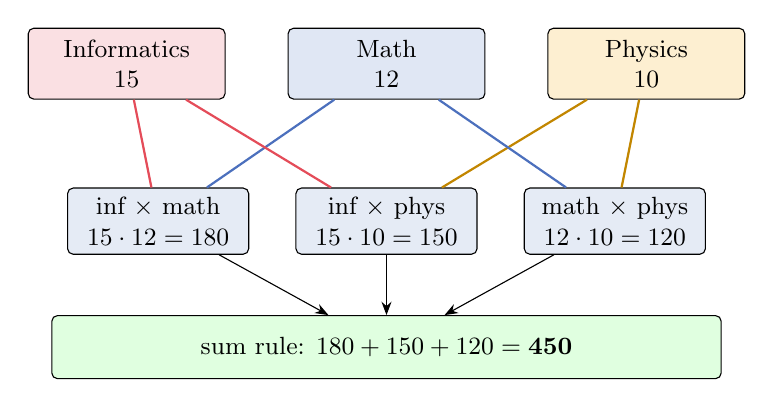
\begin{tikzpicture}[font=\small,
  pile/.style={draw, rounded corners=2pt, minimum width=2.5cm, minimum height=9mm, align=center},
  prod/.style={draw, rounded corners=2pt, minimum width=2.3cm, minimum height=8mm, align=center, fill=armBlue!10}]
% three piles
\node[pile, fill=armRed!12]    (I) at (0,0)   {Informatics\\$15$};
\node[pile, fill=armBlue!12]   (M) at (3.3,0) {Math\\$12$};
\node[pile, fill=armOrange!18] (P) at (6.6,0) {Physics\\$10$};
% the three subject-pairs and their products
\node[prod] (IM) at (0.4,-2.0)  {inf $\times$ math\\$15\cdot12=180$};
\node[prod] (IP) at (3.3,-2.0)  {inf $\times$ phys\\$15\cdot10=150$};
\node[prod] (MP) at (6.2,-2.0)  {math $\times$ phys\\$12\cdot10=120$};
\draw[armRed!70,thick]   (I) -- (IM); \draw[armBlue!70,thick]   (M) -- (IM);
\draw[armRed!70,thick]   (I) -- (IP); \draw[armOrange!80!black,thick] (P) -- (IP);
\draw[armBlue!70,thick]  (M) -- (MP); \draw[armOrange!80!black,thick] (P) -- (MP);
% sum
\node[draw, rounded corners=2pt, fill=green!12, minimum width=8.5cm, minimum height=8mm] (S) at (3.3,-3.6)
  {sum rule: $180+150+120=\mathbf{450}$};
\draw[->,>=Stealth] (IM) -- (S); \draw[->,>=Stealth] (IP) -- (S); \draw[->,>=Stealth] (MP) -- (S);
\end{tikzpicture}
\end{center}

\begin{methodbox}
\textbf{Transferable technique:} \emph{multiply within a case, add across cases.} When objects
split into disjoint types, count each type with the product rule, then sum the types (sum rule).
Choosing two of three groups always gives exactly $\binom{3}{2}=3$ cases.
\end{methodbox}

% ============================================================================
\section*{Problem 1.5 - Numbers below 700 and divisibility}

\begin{problembox}[1.5]
Among the natural numbers less than $700$: how many are divisible by $5$? Of those, how many are
also divisible by $3$? How many are divisible by both $3$ and $5$?
\end{problembox}

\begin{ideabox}
The multiples of $d$ below a bound are evenly spaced: $d,2d,3d,\dots$. So \textquotedbl{}how many
multiples of $d$ are at most $N$\textquotedbl{} is just $\lfloor N/d\rfloor$ - you fit as many full
steps of size $d$ into $N$ as you can. \textquotedbl{}Less than $700$\textquotedbl{} means
$1,2,\dots,699$, so $N=699$. The only subtlety is the last question: \textquotedbl{}divisible by
both $3$ and $5$\textquotedbl{} is the same as \textquotedbl{}divisible by $\operatorname{lcm}(3,5)=15$\textquotedbl{},
because $3$ and $5$ are coprime. And \textquotedbl{}divisible by $5$ and also by $3$\textquotedbl{}
is the very same condition - so the second and third answers coincide.
\end{ideabox}

\textbf{Step 1 - Fix the range.}
Natural numbers less than $700$ are $1,2,\dots,699$, so we use $N=699$.

\textbf{Step 2 - Divisible by $5$.}
\[
\left\lfloor \tfrac{699}{5}\right\rfloor = 139 \qquad(\text{these are } 5,10,15,\dots,695).
\]

\textbf{Step 3 - Of those, also divisible by $3$.}
A number divisible by $5$ and by $3$ is divisible by $\operatorname{lcm}(3,5)=15$ (true because
$\gcd(3,5)=1$). So count multiples of $15$:
\[
\left\lfloor \tfrac{699}{15}\right\rfloor = 46 \qquad(\text{these are } 15,30,\dots,690).
\]

\textbf{Step 4 - Divisible by both $3$ and $5$.}
This is literally the same condition - divisible by $15$ - so the count is again $46$.

\textbf{Always check.} $695 = 5\cdot 139 \le 699$ and the next multiple $700>699$, so $139$ is right.
$690 = 15\cdot 46 \le 699$ and $15\cdot 47 = 705 > 699$, so $46$ is right. \checkmark

\answer{$\lfloor 699/5\rfloor = \mathbf{139}$ divisible by $5$;\quad $\lfloor 699/15\rfloor = \mathbf{46}$ of them by $3$;\quad $\mathbf{46}$ by both $3$ and $5$.}

\begin{center}
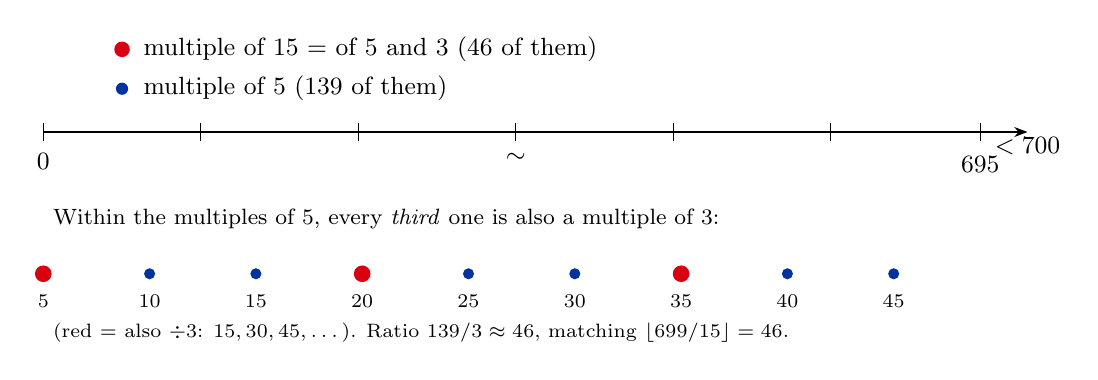
\begin{tikzpicture}[font=\small]
% number line with multiples of 5 ticked and multiples of 15 highlighted
\draw[->,>=Stealth] (0,0) -- (12.5,0) node[right]{};
\foreach \x/\lab in {0/0, 2/100, 4/200, 6/300, 8/400, 10/500, 11.9/695}{
  \draw (\x,0.12) -- (\x,-0.12);
}
\node[below] at (0,-0.15){$0$};
\node[below] at (6,-0.15){$\sim$};
\node[below] at (11.9,-0.18){$695$};
\node[below] at (12.5,0.05){$<700$};
% legend dots
\fill[armBlue] (1.0,0.55) circle (2.2pt); \node[right] at (1.15,0.55){multiple of $5$ (139 of them)};
\fill[armRed]  (1.0,1.05) circle (2.8pt); \node[right] at (1.15,1.05){multiple of $15$ = of $5$ and $3$ (46 of them)};
% small inset showing every third multiple of 5 is a multiple of 15
\node[anchor=west] at (0,-1.1)
  {\footnotesize Within the multiples of $5$, every \emph{third} one is also a multiple of $3$:};
\foreach \i in {0,...,8}{
  \pgfmathsetmacro\xx{0.0+\i*1.35}
  \ifnum\i=0 \fill[armRed](\xx,-1.8)circle(3pt);
  \else\ifnum\i=3 \fill[armRed](\xx,-1.8)circle(3pt);
  \else\ifnum\i=6 \fill[armRed](\xx,-1.8)circle(3pt);
  \else \fill[armBlue](\xx,-1.8)circle(2pt); \fi\fi\fi
  \node[below,font=\scriptsize] at (\xx,-1.95){$\pgfmathparse{int(5+\i*5)}\pgfmathresult$};
}
\node[anchor=west,font=\scriptsize] at (0.0,-2.55){(red $=$ also $\div 3$: $15,30,45,\dots$). Ratio $139/3\approx 46$, matching $\lfloor 699/15\rfloor=46$.};
\end{tikzpicture}
\end{center}

\begin{methodbox}
\textbf{Transferable technique:} the count of multiples of $d$ in $\{1,\dots,N\}$ is
$\lfloor N/d\rfloor$. \textquotedbl{}Divisible by $a$ and by $b$\textquotedbl{} collapses to
\textquotedbl{}divisible by $\operatorname{lcm}(a,b)$\textquotedbl{}; for coprime $a,b$ that is
just $a\cdot b$.
\end{methodbox}

% ============================================================================
\section*{Problem 1.10 - Seven-digit numbers with a parity pattern}

\begin{problembox}[1.10]
How many $7$-digit numbers have an \textbf{odd} digit in every \textbf{even} position and an
\textbf{even} digit in every \textbf{odd} position? (Position $1$ is the leading digit and cannot
be $0$.)
\end{problembox}

\begin{ideabox}
A $7$-digit number is just seven slots filled left to right, and each slot's digit is chosen
\emph{independently} of the others, so this is a pure product-rule count: multiply the number of
allowed digits in each slot. Read the rule slot by slot. Odd positions $1,3,5,7$ want an
\emph{even} digit, of which there are five: $\{0,2,4,6,8\}$. Even positions $2,4,6$ want an
\emph{odd} digit, also five: $\{1,3,5,7,9\}$. The single catch is the very first slot: it is an
odd position, so it wants an even digit, but it may not be $0$ (else the number is not really
$7$-digit). That removes exactly one option, leaving $\{2,4,6,8\}$, i.e. $4$ choices. Every other
slot keeps its full $5$.
\end{ideabox}

\textbf{Step 1 - Classify the slots.}
Positions $1$ to $7$. \emph{Odd} positions $\{1,3,5,7\}$ take an even digit; \emph{even} positions
$\{2,4,6\}$ take an odd digit.

\textbf{Step 2 - Count the choices per slot.}
Even digits $\{0,2,4,6,8\}$: $5$ each. Odd digits $\{1,3,5,7,9\}$: $5$ each. Position $1$ is
special: even digit but not $0$, so $\{2,4,6,8\}$, only $4$ choices.

\textbf{Step 3 - Multiply (product rule).}
One slot with $4$ choices (position $1$), and the other six slots with $5$ choices each:
\[
\underbrace{4}_{\text{pos }1}\;\cdot\;\underbrace{5\cdot5\cdot5}_{\text{pos }3,5,7}\;\cdot\;\underbrace{5\cdot5\cdot5}_{\text{pos }2,4,6}
= 4\cdot 5^{6} = 4\cdot 15625 = 62500 .
\]

\textbf{Always check.} If position $1$ could also be $0$ we would get $5^7=78125$; the
ban on a leading $0$ removes exactly the numbers with $0$ in slot $1$, which is a $\tfrac15$ share,
leaving $\tfrac45\cdot 5^7 = 4\cdot 5^6 = 62500$. Same number, reached a second way. \checkmark

\answer{$4\cdot 5^{6} = \mathbf{62500}$}

\begin{center}
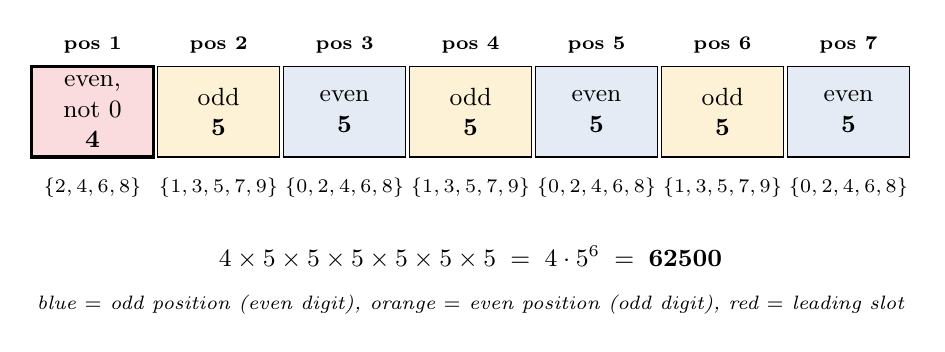
\begin{tikzpicture}[font=\small,
  slot/.style={draw, minimum width=1.55cm, minimum height=1.15cm, align=center},
  odd/.style={slot, fill=armBlue!10},   % odd position -> even digit
  evn/.style={slot, fill=armOrange!16}, % even position -> odd digit
  first/.style={slot, fill=armRed!14, very thick}]
\node[first] (p1) at (0,0)   {even,\\not $0$\\\textbf{4}};
\node[evn]   (p2) at (1.6,0) {odd\\\textbf{5}};
\node[odd]   (p3) at (3.2,0) {even\\\textbf{5}};
\node[evn]   (p4) at (4.8,0) {odd\\\textbf{5}};
\node[odd]   (p5) at (6.4,0) {even\\\textbf{5}};
\node[evn]   (p6) at (8.0,0) {odd\\\textbf{5}};
\node[odd]   (p7) at (9.6,0) {even\\\textbf{5}};
\foreach \i/\x in {1/0,2/1.6,3/3.2,4/4.8,5/6.4,6/8.0,7/9.6}{
  \node[above,font=\scriptsize\bfseries] at (\x,0.62){pos \i};
}
% digit-set reminders
\node[below,font=\scriptsize,align=center] at (0,-0.72){$\{2,4,6,8\}$};
\node[below,font=\scriptsize,align=center] at (1.6,-0.72){$\{1,3,5,7,9\}$};
\node[below,font=\scriptsize,align=center] at (3.2,-0.72){$\{0,2,4,6,8\}$};
\node[below,font=\scriptsize,align=center] at (4.8,-0.72){$\{1,3,5,7,9\}$};
\node[below,font=\scriptsize,align=center] at (6.4,-0.72){$\{0,2,4,6,8\}$};
\node[below,font=\scriptsize,align=center] at (8.0,-0.72){$\{1,3,5,7,9\}$};
\node[below,font=\scriptsize,align=center] at (9.6,-0.72){$\{0,2,4,6,8\}$};
% product line
\node[anchor=center,font=\small] at (4.8,-1.85)
  {$4\times 5\times 5\times 5\times 5\times 5\times 5 \;=\; 4\cdot 5^{6} \;=\; \mathbf{62500}$};
\node[anchor=center,font=\scriptsize\itshape] at (4.8,-2.45)
  {blue $=$ odd position (even digit), orange $=$ even position (odd digit), red $=$ leading slot};
\end{tikzpicture}
\end{center}

\begin{methodbox}
\textbf{Transferable technique:} for \textquotedbl{}fill the slots\textquotedbl{} problems where
each position is chosen independently, multiply the per-slot option counts. Handle the leading-digit
\textquotedbl{}no $0$\textquotedbl{} restriction by reducing that one slot's count.
\end{methodbox}

% ============================================================================
\section*{Problem 2.5 - Six boys and seven girls in a row, ends are boys}

\begin{problembox}[2.5]
Six boys and seven girls ($13$ distinct people) stand in a row of $13$ places. In how many ways
can they line up so that the \textbf{first and the last} place are both occupied by boys?
\end{problembox}

\begin{ideabox}
Order matters (a row), so this is an arrangement count. The clean move is to \emph{seat the
constrained spots first}: place the two end positions, which are forced to be boys, before
anything else. Choose the boy on the left end ($6$ choices), then the boy on the right end ($5$
choices left), so $6\cdot 5$ ways for the two ends. Now the two ends are settled and the
restriction is fully used up: the remaining $11$ people (the other $4$ boys and all $7$ girls)
are completely free to fill the middle $11$ places in any order, which is $11!$ ways. Multiply
the independent stages.
\end{ideabox}

\textbf{Step 1 - Fill the ends (the only restriction).}
Left end: any of the $6$ boys. Right end: any of the remaining $5$ boys. That is $6\cdot 5 = 30$
ordered ways - this is the arrangement $A_6^2 = 6\cdot 5$.

\textbf{Step 2 - Fill the middle freely.}
After the ends are fixed, $11$ distinct people remain for $11$ middle places: $11!$ orderings.

\textbf{Step 3 - Multiply (product rule).}
\[
6\cdot 5\cdot 11! = 30\cdot 39\,916\,800 = 1\,197\,504\,000 .
\]

\textbf{Always check.} Total arrangements with no restriction would be $13!$. Our condition forces
both ends to be among the $6$ boys; the fraction of all $13!$ lineups with a boy at each end is
$\tfrac{6}{13}\cdot\tfrac{5}{12}$, giving $13!\cdot\tfrac{6\cdot5}{13\cdot12} = \tfrac{13!}{156}\cdot30$.
Since $13! = 6\,227\,020\,800$, this is $6\,227\,020\,800\cdot\tfrac{30}{156}=1\,197\,504\,000$. Same number. \checkmark

\answer{$6\cdot 5\cdot 11! = 30\cdot 11! = \mathbf{1\,197\,504\,000}$}

\begin{center}
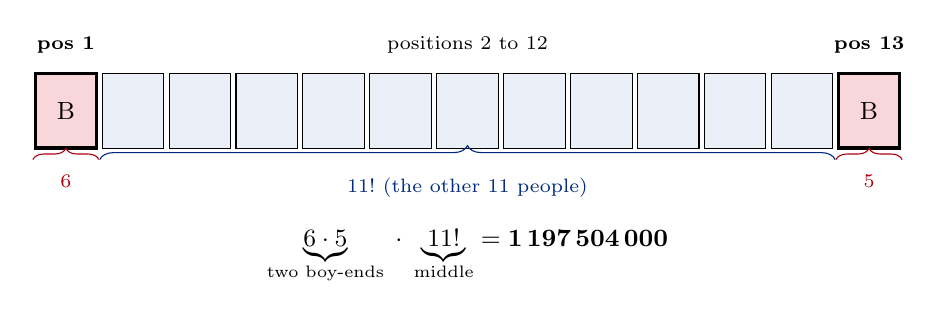
\begin{tikzpicture}[font=\small,
  box/.style={draw, minimum width=0.78cm, minimum height=0.95cm},
  endb/.style={box, fill=armRed!16, very thick},
  mid/.style={box, fill=armBlue!8}]
\node[endb] (e1) at (0,0) {B};
\foreach \i in {1,...,11}{
  \node[mid] (m\i) at (\i*0.85,0) {};
}
\node[endb] (e2) at (12*0.85,0) {B};
% labels
\node[above,font=\scriptsize\bfseries] at (0,0.6){pos 1};
\node[above,font=\scriptsize\bfseries] at (12*0.85,0.6){pos 13};
\node[above,font=\scriptsize] at (6*0.85,0.6){positions $2$ to $12$};
% braces
\draw[decorate,decoration={brace,amplitude=4pt},armRed!80!black]
  (-0.42,-0.62) -- (0.42,-0.62) node[midway,below,font=\scriptsize,yshift=-2pt]{$6$};
\draw[decorate,decoration={brace,amplitude=4pt},armRed!80!black]
  (12*0.85-0.42,-0.62) -- (12*0.85+0.42,-0.62) node[midway,below,font=\scriptsize,yshift=-2pt]{$5$};
\draw[decorate,decoration={brace,amplitude=5pt},armBlue!80!black]
  (0.85-0.42,-0.62) -- (11*0.85+0.42,-0.62) node[midway,below,font=\scriptsize,yshift=-3pt]{$11!$ (the other 11 people)};
\node[font=\small] at (6*0.85,-1.85){$\underbrace{6\cdot 5}_{\text{two boy-ends}}\;\cdot\;\underbrace{11!}_{\text{middle}}=\mathbf{1\,197\,504\,000}$};
\end{tikzpicture}
\end{center}

\begin{methodbox}
\textbf{Transferable technique:} \emph{place the restricted positions first}, then arrange the
rest freely. Choosing ordered people for $k$ named spots out of $n$ is $A_n^k = n(n-1)\cdots(n-k+1)$;
the leftover $n-k$ people fill the remaining spots in $(n-k)!$ ways.
\end{methodbox}

% ============================================================================
\section*{Problem 2.10 - Three mutual friends or three mutual strangers}

\begin{problembox}[2.10]
In a room of $6$ people, every two of them are either \textbf{friends} or \textbf{strangers}.
Prove that there are always three people who are pairwise friends, or three people who are
pairwise strangers.
\end{problembox}

\begin{ideabox}
Model it as a complete graph $K_6$: $6$ dots, one edge between every pair, each edge coloured
\textbf{red} (friends) or \textbf{blue} (strangers). The claim is that some triangle is
monochromatic. The trick is to look from \emph{one} person $P$. $P$ has $5$ edges; two colours;
by the \textbf{pigeonhole principle} at least $\lceil 5/2\rceil = 3$ of them share a colour - say
$P$ is friends (red) with three people $A,B,C$. Now everything hinges on the triangle $A,B,C$.
If even one of the pairs $AB,BC,CA$ is red, that pair plus $P$ is an all-red triangle (three mutual
friends). If \emph{none} of them is red, then $AB,BC,CA$ are all blue, so $A,B,C$ themselves are an
all-blue triangle (three mutual strangers). There is no escape. This is exactly the statement
$R(3,3)\le 6$.
\end{ideabox}

\textbf{Step 1 - Set up the model.}
Vertices $=$ the $6$ people; colour each of the $\binom{6}{2}=15$ edges red (friends) or blue
(strangers). \textquotedbl{}Three mutual friends\textquotedbl{} $=$ a red triangle; \textquotedbl{}three
mutual strangers\textquotedbl{} $=$ a blue triangle.

\textbf{Step 2 - Pigeonhole at one vertex.}
Fix any person $P$. The $5$ edges leaving $P$ are coloured with $2$ colours, and
$\lceil 5/2\rceil=3$, so by pigeonhole at least $3$ of them have the same colour. Without loss of
generality, $P$ is joined in \textbf{red} to three people $A,B,C$ (if instead the majority colour
is blue, swap the words \textquotedbl{}friends\textquotedbl{}/\textquotedbl{}strangers\textquotedbl{}
throughout - the argument is identical).

\textbf{Step 3 - Examine the triangle $A,B,C$ (two cases).}
\begin{itemize}[leftmargin=1.3em,topsep=2pt]
\item \emph{Some edge among $A,B,C$ is red}, say $AB$. Then $P\!A$, $P\!B$, $AB$ are all red:
$P,A,B$ are three mutual friends. Done.
\item \emph{No edge among $A,B,C$ is red.} Then $AB$, $BC$, $CA$ are all blue, so $A,B,C$ are
three mutual strangers. Done.
\end{itemize}
One of the two cases must occur, so a monochromatic triangle always exists. $\blacksquare$

\textbf{Always check (is $6$ the right number?).} With only $5$ people the claim can fail: colour
$K_5$ as a red $5$-cycle and a blue $5$-cycle (the \textquotedbl{}pentagon and
pentagram\textquotedbl{}) and no triangle is monochromatic. So $5$ is not enough and $6$ is sharp;
that is why the problem says $6$. (Brute force confirms: among all $2^{15}$ colourings of $K_6$,
\emph{zero} avoid a monochromatic triangle, while $K_5$ has colourings that do.) \checkmark

\answer{Such a monochromatic triangle always exists: this is $R(3,3)\le 6$.}

\begin{center}
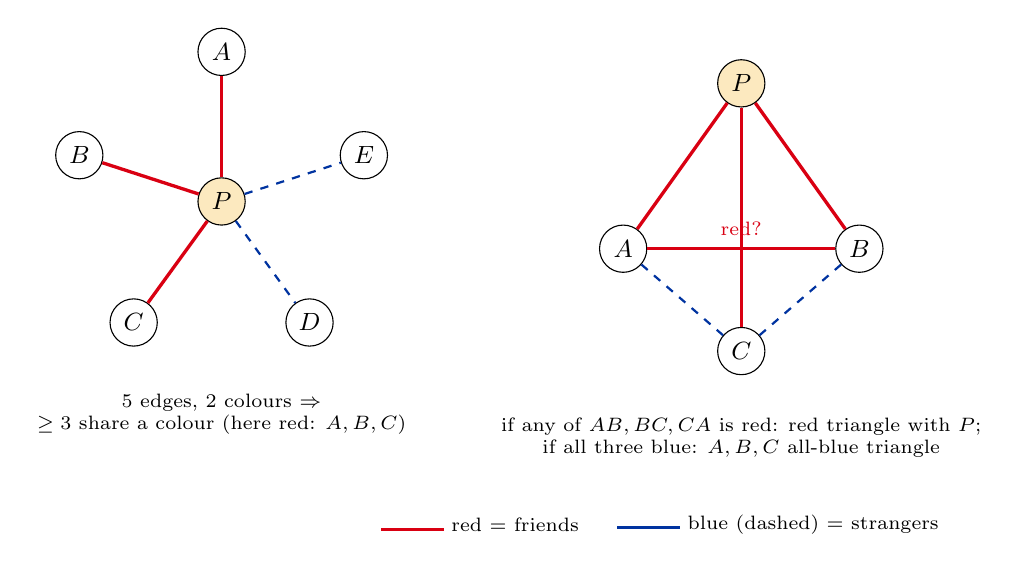
\begin{tikzpicture}[font=\small, scale=1.0,
  ppl/.style={circle, draw, fill=white, inner sep=1.3pt, minimum size=6mm, font=\small\bfseries}]
% Left picture: P with 5 edges, 3 red by pigeonhole
\begin{scope}[xshift=-3.2cm]
\node[ppl, fill=armOrange!25] (P) at (0,0) {$P$};
\node[ppl] (A) at (90:1.9)  {$A$};
\node[ppl] (B) at (162:1.9) {$B$};
\node[ppl] (C) at (234:1.9) {$C$};
\node[ppl] (D) at (306:1.9) {$D$};
\node[ppl] (E) at (18:1.9)  {$E$};
% 3 red edges P-A,P-B,P-C ; 2 other edges blue (P-D, P-E)
\draw[armRed,very thick] (P)--(A);
\draw[armRed,very thick] (P)--(B);
\draw[armRed,very thick] (P)--(C);
\draw[armBlue,thick,dashed] (P)--(D);
\draw[armBlue,thick,dashed] (P)--(E);
\node[font=\scriptsize, align=center] at (0,-2.7)
  {$5$ edges, $2$ colours $\Rightarrow$\\ $\ge 3$ share a colour (here red: $A,B,C$)};
\end{scope}
% Right picture: triangle ABC case split
\begin{scope}[xshift=3.4cm]
\node[ppl, fill=armOrange!25] (P2) at (0,1.5) {$P$};
\node[ppl] (A2) at (-1.5,-0.6) {$A$};
\node[ppl] (B2) at (1.5,-0.6)  {$B$};
\node[ppl] (C2) at (0,-1.9)    {$C$};
\draw[armRed,very thick] (P2)--(A2);
\draw[armRed,very thick] (P2)--(B2);
\draw[armRed,very thick] (P2)--(C2);
% the three ABC edges: if any is red -> red triangle with P; else all blue -> blue triangle ABC
\draw[armRed,very thick] (A2)--(B2) node[midway,above,font=\scriptsize,yshift=1pt]{red?};
\draw[armBlue,thick,dashed] (B2)--(C2);
\draw[armBlue,thick,dashed] (C2)--(A2);
\node[font=\scriptsize, align=center] at (0,-3.0)
  {if any of $AB,BC,CA$ is red: red triangle with $P$;\\ if all three blue: $A,B,C$ all-blue triangle};
\end{scope}
% legend
\node[font=\scriptsize, anchor=west] at (-1.3,-4.1) {\textcolor{armRed}{\rule{8mm}{1.1pt}} red = friends};
\node[font=\scriptsize, anchor=west] at (1.7,-4.1) {\textcolor{armBlue}{\rule{8mm}{1.1pt}} blue (dashed) = strangers};
\end{tikzpicture}
\end{center}

\begin{methodbox}
\textbf{Transferable technique (Ramsey via pigeonhole):} to force structure, focus on one vertex,
pigeonhole its edges into a majority colour, then check the small group that majority creates. The
two-case split \textquotedbl{}some edge inside is colour $X$\textquotedbl{} vs
\textquotedbl{}none is\textquotedbl{} is the engine. This proves $R(3,3)\le 6$.
\end{methodbox}

% ============================================================================
\section*{Problem 2.12 - One of $7,77,777,\dots$ is divisible by $2013$}

\begin{problembox}[2.12]
Consider the sequence $7,\,77,\,777,\,7777,\dots$ (term $n$ is the number written with $n$
sevens). Prove that among its first $2014$ terms, at least one is divisible by $2013$.
\end{problembox}

\begin{ideabox}
You cannot point to which term works without computing, but you do not need to - you only need to
prove one \emph{exists}. The tool is the \textbf{pigeonhole principle} applied to remainders. Look
at the first $2014$ terms modulo $2013$. A remainder mod $2013$ is one of only $2013$ values
$\{0,1,\dots,2012\}$ - that is $2013$ \textquotedbl{}boxes\textquotedbl{}. But we have $2014$ terms
to drop into them, so two terms must land in the same box, i.e. share a remainder. Their
\emph{difference} is then divisible by $2013$. The last step is to see that this difference is
itself a number of the right shape (sevens followed by zeros), and the zeros (a power of $10$) can
be stripped off because $2013$ is coprime to $10$. What remains is a term of the sequence divisible
by $2013$.
\end{ideabox}

\textbf{Step 1 - Set up boxes and objects.}
Let $a_n = \underbrace{77\cdots7}_{n\text{ sevens}}$. Look at the remainders
$a_1 \bmod 2013,\ a_2\bmod 2013,\ \dots,\ a_{2014}\bmod 2013$. Each remainder is one of the
$2013$ values $0,1,\dots,2012$.

\textbf{Step 2 - Pigeonhole.}
We have $2014$ remainders but only $2013$ possible values, so two of them are equal:
\[
a_i \equiv a_j \pmod{2013},\qquad \text{for some } 1\le i < j \le 2014 .
\]
(If instead one of the remainders is already $0$, that term is divisible by $2013$ and we are
done immediately.)

\textbf{Step 3 - The difference is divisible by $2013$.}
From $a_i\equiv a_j$ we get $2013 \mid (a_j - a_i)$. Subtracting the two repunits-of-sevens:
\[
a_j - a_i = \underbrace{77\cdots7}_{j} - \underbrace{77\cdots7}_{i}
= \underbrace{77\cdots7}_{\,j-i\,}\underbrace{00\cdots0}_{\,i\,}
= a_{\,j-i}\cdot 10^{\,i}.
\]
(The top $j-i$ sevens survive; the bottom $i$ digits cancel to zeros.)

\textbf{Step 4 - Strip the power of $10$.}
$2013 = 3\cdot 11\cdot 61$, which shares no factor with $10=2\cdot 5$, so $\gcd(2013,10^{\,i})=1$.
Since $2013 \mid a_{\,j-i}\cdot 10^{\,i}$ and $2013$ is coprime to $10^{\,i}$, it must divide the
other factor:
\[
2013 \mid a_{\,j-i}.
\]
Finally $1 \le j-i \le 2013 < 2014$, so $a_{\,j-i}$ is one of the first $2014$ terms. $\blacksquare$

\textbf{Always check.} The proof only guarantees \emph{existence}; a direct computation shows the
first term that actually works is $a_{60}$ (the number with sixty $7$s), and indeed $60 \le 2014$.
So the existence claim is not just true but comfortably so. \checkmark

\answer{Some $a_{j-i}$ with $1\le j-i\le 2013$ is divisible by $2013$; in fact $a_{60}$ already is.}

\begin{center}
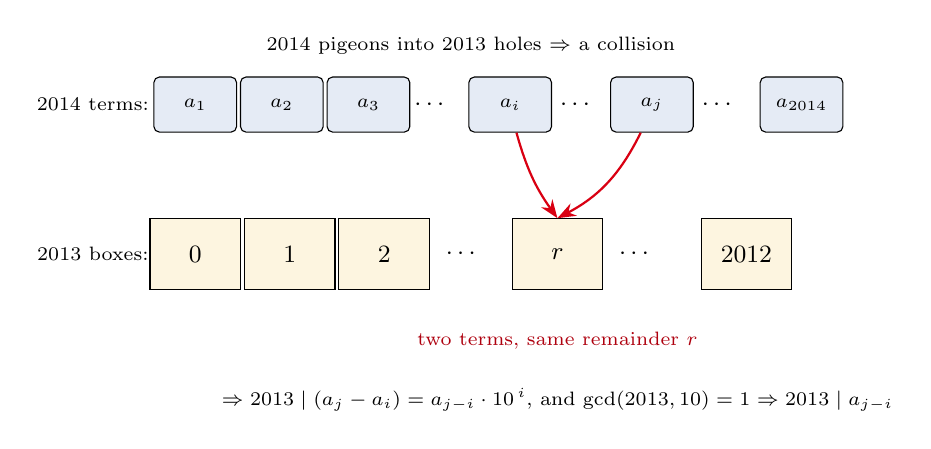
\begin{tikzpicture}[font=\small,
  trm/.style={draw, rounded corners=2pt, minimum width=1.05cm, minimum height=7mm, fill=armBlue!10, font=\scriptsize},
  box/.style={draw, minimum width=1.15cm, minimum height=9mm, fill=armOrange!12}]
% top row: 2014 terms (show a few then dots)
\node[font=\scriptsize] at (-1.3,1.6) {$2014$ terms:};
\node[trm] (t1) at (0,1.6) {$a_1$};
\node[trm] (t2) at (1.1,1.6) {$a_2$};
\node[trm] (t3) at (2.2,1.6) {$a_3$};
\node at (3.0,1.6) {$\cdots$};
\node[trm] (tk) at (4.0,1.6) {$a_i$};
\node at (4.85,1.6) {$\cdots$};
\node[trm] (tl) at (5.8,1.6) {$a_j$};
\node at (6.65,1.6) {$\cdots$};
\node[trm] (tn) at (7.7,1.6) {$a_{2014}$};
% boxes: 2013 remainder boxes
\node[font=\scriptsize] at (-1.3,-0.3) {$2013$ boxes:};
\node[box] (b0) at (0,-0.3) {$0$};
\node[box] (b1) at (1.2,-0.3) {$1$};
\node[box] (b2) at (2.4,-0.3) {$2$};
\node at (3.4,-0.3) {$\cdots$};
\node[box] (br) at (4.6,-0.3) {$r$};
\node at (5.6,-0.3) {$\cdots$};
\node[box] (be) at (7.0,-0.3) {$2012$};
% two terms a_i, a_j land in same box r
\draw[->,>=Stealth,armRed,thick] (tk) to[bend right=10] (br.north);
\draw[->,>=Stealth,armRed,thick] (tl) to[bend left=18] (br.north);
\node[font=\scriptsize,armRed!80!black,align=center] at (4.6,-1.4)
  {two terms, same remainder $r$};
\node[font=\scriptsize,align=center] at (4.6,-2.15)
  {$\Rightarrow 2013\mid(a_j-a_i)=a_{j-i}\cdot 10^{\,i}$, and $\gcd(2013,10)=1\Rightarrow 2013\mid a_{j-i}$};
\node[font=\scriptsize] at (3.5,2.35) {$2014$ pigeons into $2013$ holes $\Rightarrow$ a collision};
\end{tikzpicture}
\end{center}

\begin{methodbox}
\textbf{Transferable technique:} to show \textquotedbl{}some term is divisible by $m$,\textquotedbl{}
take $m+1$ candidates and pigeonhole their remainders mod $m$; a repeat gives a difference divisible
by $m$. If the difference carries a factor $10^{k}$, drop it using $\gcd(m,10)=1$.
\end{methodbox}

\end{document}
